\pagecolor{CadetBlue!70!green}
\chapter{Eine kurze Einführung zum Arduino und zu Nepo}
\label{kap:nepo}

Der Arduino ist ein Mikrocontroller, der vom italienischen Professor Massimo Banzi entwickelt wurde, damit seine Studenten im Bereich \emph{Design} eine einfach zugängliche Möglichkeit fanden, Elektronik für künstlerische Projekte zu nutzen. Die vorgenommenen Vereinfachungen in der Handhabung von Mikrocontrollern gefielen jedoch nicht nur den Studenten von Massimo Banzi, sondern auch zahlreichen Studenten anderer Fachrichtungen, Schülern, Hobby-Elektronikern und sogar Fachleuten in der Industrie, sodass der Arduino rasch eine weltweite Verbreitung fand.

\bigskip
In diesem Kapitel lernst du\dots
\begin{itemize}
	\item \dots wie der Arduino aufgebaut ist,
	\item \dots wie man den Arduino mit dem PC verbindet und mit Nepo im Open Roberta Lab programmiert,
	\item \dots die digitalen Pins als Ausgänge zu benutzen, um eine LED zu steuern,
	\item \dots Schaltungen auf dem Steckbrett aufzubauen.
\end{itemize}

\bigskip

\bigskip

\begin{projektueberblick}
	\item Ampel \dotfill \pageref{proj:ampel}
	\item Augentestgerät \dotfill\pageref{proj:augentest}
\end{projektueberblick}

\newpage
\nopagecolor
\section{Der Aufbau des Arduino UNO}
Mit der Zeit entwickelten sich zahlreiche andere Modelle des Arduino, die kleiner oder größer waren, über mehr oder weniger Anschlüsse verfügten, schneller oder langsamer waren usw. Das Standardmodell ist heute der Arduino Uno, den auch wir verwenden.

\begin{figure}[h]
	\centering
	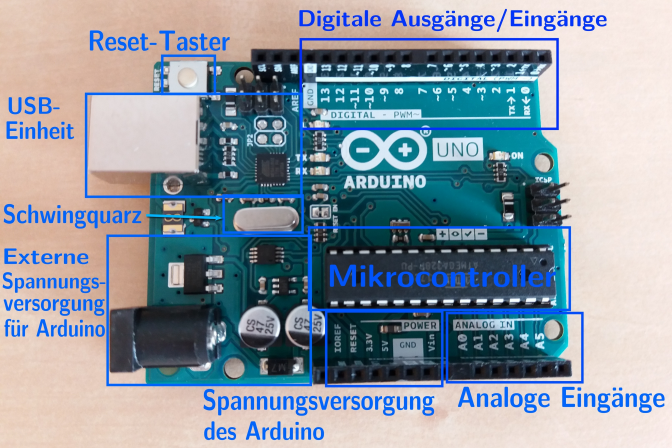
\includegraphics[width=0.8\textwidth]{pics/arduino-beschriftet.png}
	\caption{Die wichtigsten Komponenten eines Arduino Uno.}
	\label{abb:arduino-beschriftet}
\end{figure}

Abbildung \ref{abb:arduino-beschriftet} zeigt die wichtigsten Komponenten des Arduino Uno. Eine genauere Beschreibung dieser Funktionseinheiten und ihrer spezifischen Eigenschaften findet sich in Anhang \ref{sec:ueberblick}. Wichtig sind an dieser Stelle vor allem folgende Punkte:
\begin{itemize}
	\item Über den USB-Anschluss und das mitgelieferte Kabel lässt sich der Arduino mit dem PC verbinden und programmieren.
	\item Das Programm läuft nach dem Übertragen auf dem eigentlichen Mikrocontroller, dem langen schwarzen Ding in der Mitte. Der ganze Rest auf dieser kleinen Platine dient der einfacheren Handhabung des Mikrocontrollers.
	\item An den Seiten befinden sich die Pin-Leisten, an die sich zum Beispiel LEDs anschließen lassen. Die Pins sind durchnummeriert, sodass sie im Programm angesprochen werden können. \emph{GND} steht für \enquote{Ground} oder den Minus-Kontakt. \emph{5V} steht für den Plus-Kontakt und gibt an, dass dort stets eine Spannung von 5V anliegt, wenn der Arduino über USB oder Batterie mit Strom versorgt wird. Die durchnummerierten Digitalpins können durch das Programm ebenfalls auf 5V gesetzt werden (\texttt{HIGH}), aber auch auf 0V, sodass kein Strom fließt (\texttt{LOW}).
\end{itemize}
\vfill

\section{Das Open Roberta Lab und Nepo4Arduino}

Nepo4Arduino ist eine graphische Programmiersprache, die vom Fraunhofer Institut für Intelligente Analyse- und Informationssysteme im Rahmen des Open Roberta Labs für verschiedene Robotersysteme entwickelt wird. Durch die bereit gestellten Blöcke wird der Einstieg in die Programmierung des Arduino sehr einfach gemacht. Gleichzeitig lassen sich aber auch sehr komplexe Programme entwickeln und man kann jederzeit das textbasierte Programm in der Sprache C++ einsehen.

Um den Arduino zu programmieren, ruft man die Adresse \url{https://lab.open-roberta.org/} auf und wählt dann $\infty$ \texttt{Nepo4Arduino} und im nächsten Schritt den Arduino Uno aus. Damit das dort erstellte Programm aus dem Browser auf den Arduino übertragen werden kann, muss außerdem der \texttt{Open Roberta Connector} installiert werden. Auf der \href{https://jira.iais.fraunhofer.de/wiki/display/ORInfo/Open+Roberta+Wiki}{Wiki-Seite} gibt es eine \href{https://jira.iais.fraunhofer.de/wiki/display/ORInfo/Open+Roberta+Connector}{Installations-Anleitung} und eine \href{https://jira.iais.fraunhofer.de/wiki/display/ORInfo/Vorbereitung+Nepo4Arduino}{Anleitung zum Verbinden des Arduino mit dem Open Roberta Lab}.

Abbildung \ref{abb:openrobertalab} zeigt eine Übersicht über die Oberfläche des Open Roberta Lab, jedoch lernt man sie am besten kennen, indem man einfach drauf loslegt und ausprobiert, was sich damit anstellen lässt.

\begin{figure}[H]
	\centering
	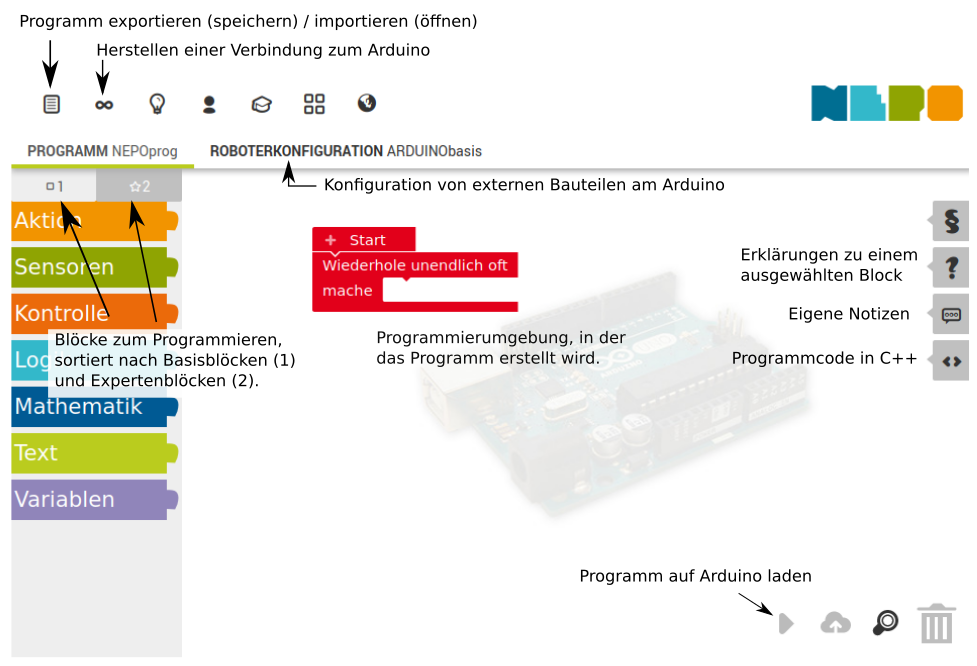
\includegraphics[width=\textwidth]{./pics/openrobertalab.png}
	\caption{Übersicht über die Funktionen von Open Roberta Lab.}
	\label{abb:openrobertalab}
\end{figure}

\newpage
\section{Digitale Ausgänge steuern}

\begin{ziel}
	\textbf{Ziel:} Es soll das erste Testprogramm auf den Arduino übertragen werden, mit dem man üblicherweise überprüft, ob der Arduino (oder ein anderer Mikrocontroller) richtig funktioniert.
\end{ziel}

\begin{aufgabe} \emph{Test der Funktionsweise}
	
	Zum Testen der Funktionsweise soll die bordeigene LED zum Blinken gebracht werden:
	\begin{itemize}[itemsep=0ex]
		\item Stelle LED an.
		\item Warte eine Sekunde.
		\item Stelle LED aus.
		\item Warte eine Sekunde.
	\end{itemize}
	
	\begin{enumerate}[label= \alph*), itemsep=0ex, parsep=0ex]
		\item Verbinde den Arduino mit dem Open Roberta Lab nach der \href{https://jira.iais.fraunhofer.de/wiki/display/ORInfo/Vorbereitung+Nepo4Arduino}{Anleitung zum Verbinden des Arduino}.
		\item Überprüfe zunächst in der Roboterkonfiguration, ob der Block für die Board-LED bereits eingestellt ist. Benenne die LED als \enquote{BoardLED}.
		\item Erstelle das oben formulierte Programm mit Nepo4Arduino und übertrage es auf den Arduino.
		\item Zum Speichern des Programms wähle im ~\nepomenu\texttt{Menü} die Funktion ~\nepoexport\texttt{exportiere Programm}. Finde das Programm im Download-Ordner deines Computers und benenne es als \texttt{Blink.xml}. Speichere es dann an einem sinnvollen Ort ab.
		
		\emph{Hinweis:} Du kannst das Programm im gleichen Menü wieder importieren, um es zu einem späteren Zeitpunkt wieder aufzurufen.
	\end{enumerate}
\end{aufgabe}

\begin{zsfg}{{Algorithmus, Anweisung und Argument}}
	\begin{wrapfigure}{r}{0.3\textwidth}
		\centering
		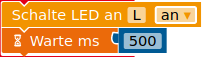
\includegraphics[width=0.3\textwidth]{./pics/anweisungen-bsp.png}
		\caption{Anweisungen und Argumente in einem Algorithmus.}
		\label{abb:befehlbsp}
	\end{wrapfigure}
	Ein Programm besteht aus einer Folge von Anweisungen. Man spricht auch von Algorithmen: Ein Algorithmus ist eine eindeutige Handlungsvorschrift zur Lösung eines Problems, die aus endlich vielen Anweisungen besteht (s. \href{https://de.wikipedia.org/wiki/Algorithmus}{Wikipedia}).
	
	Eine Anweisung \emph{kann} ein oder mehrere \emph{Argumente} haben, die zum Beispiel festlegen, welche LED geschaltet oder wie lange gewartet werden soll.
\end{zsfg}

\begin{aufgabe}
	Wir nutzen in den ersten Kapiteln sehr häufig LEDs, weil sich die Grundlagen mit ihnen einfach erarbeiten lassen, aber auch weil sie eine enorme Bedeutung in der heutigen Welt haben. Notiere dir zur Verdeutlichung eine Woche lang alle Geräte, die dir begegnen oder die dir einfallen, in denen LEDs verbaut sind.
\end{aufgabe}
\vfill

\newpage
\section{Aufbau von Schaltungen auf der Steckplatine}

In der Regel braucht man für interessante Geräte zusätzliche \emph{Hardware} (Sensoren, Motoren, \dots), die am Arduino angeschlossen wird. Bevor diese fest verlötet werden, nutzt man normalerweise Steckverbindungen bzw. baut die Schaltung auf einem kleinen Steckbrett auf, auf dem man die Verbindungen schnell wieder lösen kann, falls nötig. Steckbretter sind aus dem Physikunterricht bekannt. Abbildung \ref{abb:steckbrett} zeigt, welche Kontakte auf dem Steckbrett miteinander verbunden sind.

\begin{figure}[H]
	\centering
	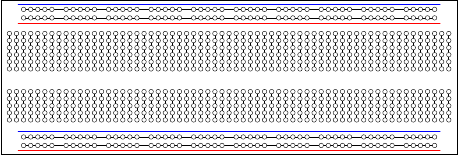
\includegraphics[width=0.8\textwidth]{./Zeichnungen/steckbrett.png}
	\caption{Die Steckverbindungen sind außen in Längsrichtung und innen in Querrichtung miteinander verbunden.}
	\label{abb:steckbrett}
\end{figure}

\begin{ziel}
	\textbf{Ziel:} Eine externe LED an Pin 13 soll zum Leuchten gebracht werden. Diese kann genutzt werden, um das Blinken einer Alarmanlagen-LED zu simulieren.
\end{ziel}

\medskip
\begin{minipage}{0.48\textwidth}
	\begin{figure}[H]
		\centering
		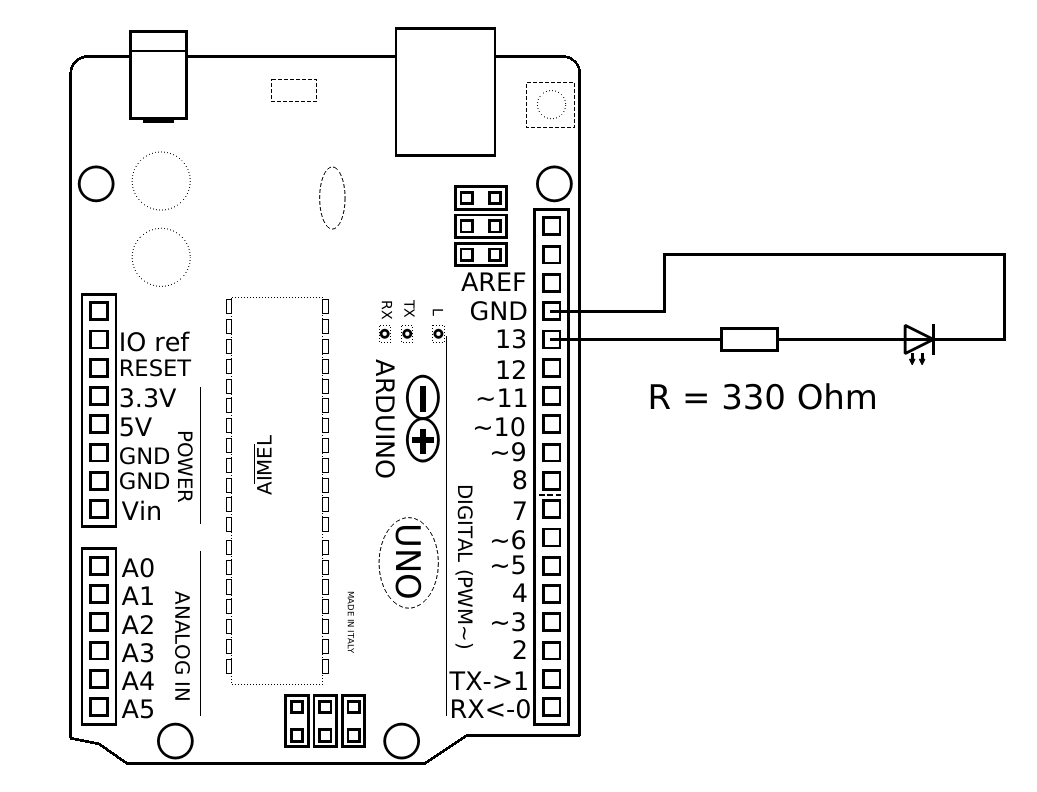
\includegraphics[width=\textwidth]{./Zeichnungen/Schaltplan-LED.png}
		\caption{Schaltplan zum Anschließen einer LED mit Vorwiderstand an Pin 13.}
	\end{figure}
\end{minipage}
\hfill
\begin{minipage}{0.5\textwidth}
	\emph{Hinweise:} 
	
	Es kann das Programm aus dem vorherigen Abschnitt wieder verwendet werden, da die Board-LED ebenfalls mit Pin 13 verbunden ist. Allerdings gibt es noch etwas zu beachten: Wenn die LED an Pin 13 angeschaltet wird, bedeutet das, dass der Arduino an Pin 13 eine Spannung von 5V (Pluspol) gegenüber GND (Minuspol) ausgibt. Die LED verträgt jedoch nur (je nach Farbe) gut 2\,V. Daher ist die LED mit einem Vorwiderstand von $\SI{330}{\SIUnitSymbolOhm}$ verbunden.
	
	Die LED ist ein sogenanntes gepoltes Bauteil. Das heißt, dass der lange Kontaktstift der LED an den Pluspol angeschlossen werden \emph{muss} und der kurze an den Minuspol (GND) angeschlossen werden \emph{muss}.
\end{minipage}
\marginpar{%
	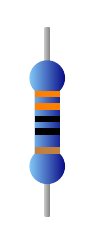
\begin{tikzpicture}[rotate=-90, scale=0.16, baseline=-1mm]
	\shade [left color=lightgray, right color=gray] (-5,0.8) rectangle (10,1.2);
	\shade [left color=LightSkyBlue, right color=NavyBlue] (0,0) -- (5,0) arc [start angle=-135, end angle=135, radius=1.414] -- (0,2) arc [start angle=45, end angle=315, radius=1.414];
	\fill [orange] (0,0) rectangle ++(0.5,2);
	\fill [orange] (1,0) rectangle ++(0.5,2);
	\fill [black] (2,0) rectangle ++(0.5,2);
	\fill [black] (3,0) rectangle ++(0.5,2);
	\fill [brown] (4.5,0) rectangle ++(0.5,2);
	\end{tikzpicture}
	\\
	
	\tiny 330 Ohm
	
	Widerstand
	\\
	\\
	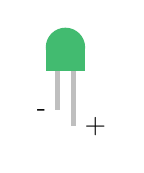
\begin{tikzpicture}[]
	\fill [CadetBlue!70!green] (0,0) circle (0.25cm); %ursprünglich gray!50!white
	\fill [CadetBlue!70!green] (-0.25,0) rectangle (0.25,-0.3);
	\draw [ultra thick, gray!50!white] (-0.1,-0.3) -- (-0.1,-0.8) node [left, black] {\sffamily -};
	\draw [ultra thick, gray!50!white] (0.1,-0.3) -- (0.1,-1) node [right, black] {\sffamily +};
	\end{tikzpicture}
	
	\tiny LED
}

\bigskip
\begin{projekt}[Ampel]\label{proj:ampel}
	Baue und programmiere eine Ampelschaltung! Verwende für die LEDs aussagekräftige Namen. Denke daran, dein Programm abzuspeichern!
	
	\emph{Für Schnelle:} Erweitere die Ampel um einen Nachtmodus.
\end{projekt}

%\bigskip
\begin{projekt}[Augentestgerät]\label{proj:augentest}
	Moderne Fernseher nutzen meist eine Bildwiederholungsrate von 144 Hertz; das bedeutet, es werden 144 Bilder pro Sekunde eingespielt. Finde mithilfe des Blink-Programms heraus, ab welchem Blinkintervall du kein Flackern mehr wahrnimmst und berechne, wie viele \enquote{Bilder} pro Sekunde sich daraus ergeben. Vergleiche diesen Wert mit der Bildwiederholungsrate im Fernsehen.
	
	{\scriptsize Idee: Frick, Fritsch und Trick (2015): \emph{Einführung in Mikrocontroller - Der Arduino als Steuerzentrale}, Bad Saulgau}
\end{projekt}

\begin{zsfg}{LED}
%	\begin{wrapfigure}{r}{0.3\textwidth}
%		\centering
%		\vspace{-0.5\baselineskip}
%		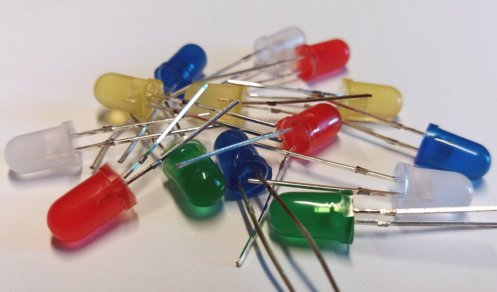
\includegraphics[width=0.3\textwidth]{./pics/led-sammlung.jpg}
%		\label{abb:led-sammlung}
%		\vspace{-\baselineskip}
%	\end{wrapfigure}
	\begin{minipage}{0.7\textwidth}
		Die Bezeichnung \enquote{LED} steht für \emph{Licht emittierende Diode} (kurz: Leuchtdiode). Sie ist ein Halbleiterbauelement, das elektrische Energie sehr effizient in Lichtenergie umwandelt und daher heute weite Verbreitung in allen Bereichen gefunden hat, in denen Licht benötigt wird. Sie ist ein gepoltes Bauteil. Das heißt, dass der lange Kontaktstift der LED mit dem Pluspol und der kurze Kontaktstift mit dem Minuspol verbunden werden muss, damit sie leuchten kann. Damit die LED nicht durchbrennt, muss in der Regel ein Vorwiderstand angebracht werden, um sie zu betreiben.
	\end{minipage}
	\hfill
	\begin{minipage}{0.28\textwidth}
%		\begin{minipage}{0.48\textwidth}
%			\centering
%			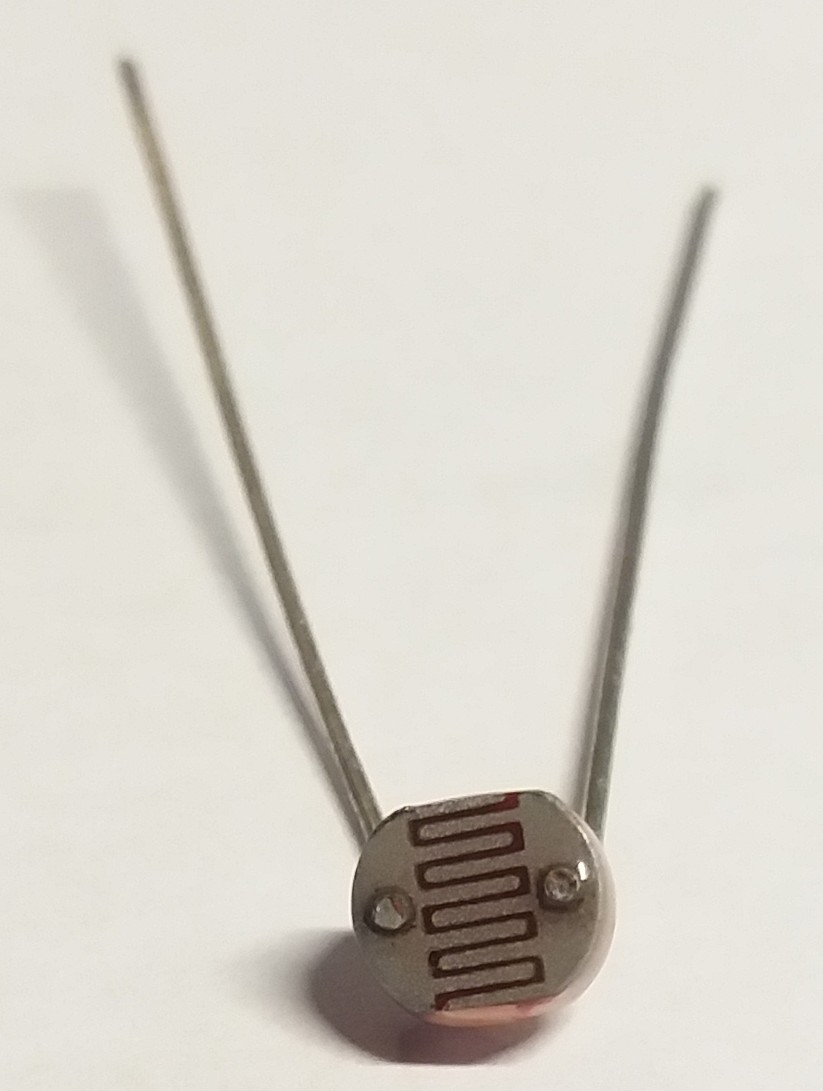
\includegraphics[width=0.9\textwidth]{./pics/ldr.jpg}
%		\end{minipage}
%		\hfill
%		\begin{minipage}{0.48\textwidth}
%			\centering
%			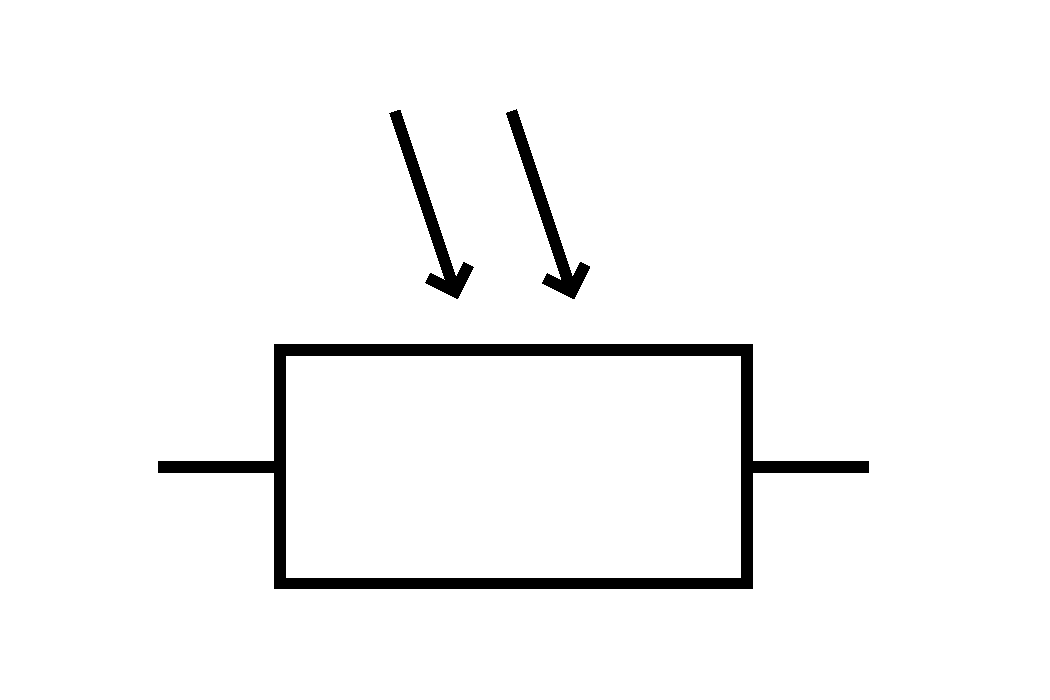
\includegraphics[width=\textwidth]{./pics/ldr-schaltsymbol.png}
%		\end{minipage}
		\centering
%		\vspace{-0.5\baselineskip}
		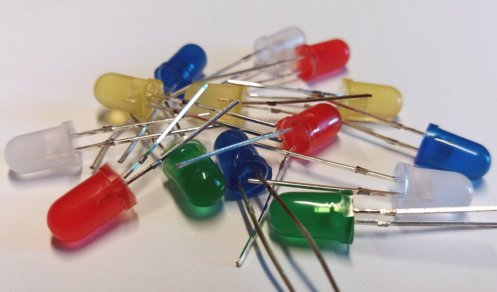
\includegraphics[width=\textwidth]{./pics/led-sammlung.jpg}
%		\label{abb:led-sammlung}
		
		\bigskip
		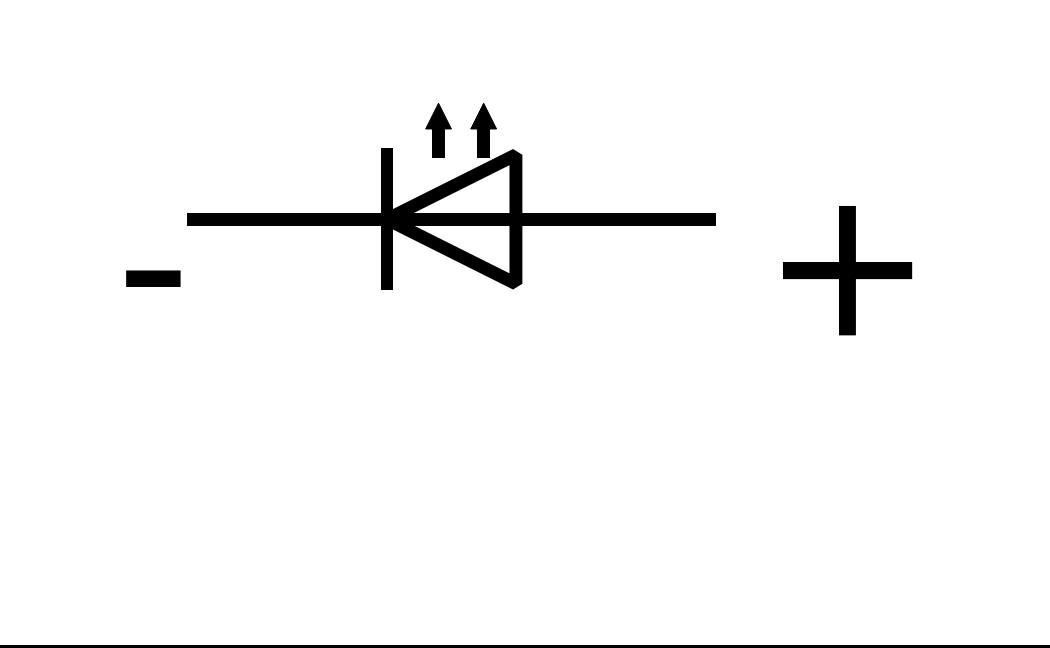
\includegraphics[width=0.7\textwidth]{./Zeichnungen/led-schaltsymbol.png}
	\end{minipage}
\end{zsfg}

\section{Widerstandsringe ablesen}
\label{sec:widerstandsringe}

Leider sind die Widerstände zu klein, um ihren Wert darauf gut lesbar zu drucken. Daher werden die Widerstände mit Ringen versehen, aus deren Farbe sich die Größe des Widerstands ablesen lässt. Um im Folgenden jeweils den passenden Widerstand aus dem Bausatz auswählen zu können, müssen wir diesen Farbcode lesen können.

Bei den blauen Kohleschichtwiderständen, die wir verwenden, gibt es fünf Ringe und jede Ringfarbe steht für eine Zahl. Die ersten drei Ringe bilden die ersten drei Ziffern des Widerstandswertes ab. Die darauf folgende Ringfarbe steht für die Zehnerpotenz, die mit den drei Ziffern multipliziert werden muss. Dies dient dazu, auch größere Widerstandswerte codieren zu können. Der letzte Ring wiederum soll einen etwas größeren Abstand haben und steht für die Fehlertoleranz des Widerstandswertes. In der Praxis lässt sich allerdings nicht immer gut erkennen, welcher Ring der letzte und welcher der erste ist\dots

\begin{figure}[H]
	\centering
	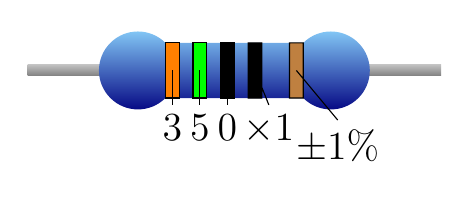
\begin{tikzpicture}[scale=0.35]
	\shade [top color=lightgray, bottom color=gray] (-5,0.8) rectangle (10,1.2);
	\shade [top color=LightSkyBlue, bottom color=NavyBlue] (0,0) -- (5,0) arc [start angle=-135, end angle=135, radius=1.414] -- (0,2) arc [start angle=45, end angle=315, radius=1.414];
	\draw [fill=orange] (0,0) rectangle ++(0.5,2) ++(-0.25,-1) -- ++(0,-1.25) [anchor =north] node {\Large 3};
	\draw [fill=green] (1,0) rectangle ++(0.5,2) ++(-0.25,-1) -- ++(0,-1.25) [anchor =north] node {\Large 5};
	\draw [fill=black] (2,0) rectangle ++(0.5,2) ++(-0.25,-1) -- ++(0,-1.25) [anchor =north] node {\Large 0};
	\draw [fill=black] (3,0) rectangle ++(0.5,2) ++(-0.25,-1) -- ++(0.5,-1.25) [anchor =north] node {\Large $\times 1$};
	\draw [fill=brown] (4.5,0) rectangle ++(0.5,2) ++(-0.25,-1) -- ++(1.5,-1.8) [anchor =north] node {\Large $\pm1\%$};
	\end{tikzpicture}
\end{figure}
Ein Beispiel: Die Ringfarben lauten orange - grün - schwarz - schwarz - braun. Anhand der folgenden Tabelle lässt sich daraus der Wert konstruieren: $3 - 5 - 0 - \cdot 1 (=10^0) - \pm 1\% $, kurz: $\SI{350}{\SIUnitSymbolOhm}\pm\SI{3,5}{\SIUnitSymbolOhm}$.

\begin{table}[H]
	\centering
	%\rowcolors{1}{lightgray}{white}
	\begin{minipage}[c]{\textwidth}
		\begin{tabu} to \textwidth {X[L,2]X[C]X[C]X[C]X[C,3]X[C,2]}
			\toprule
			\textbf{Ringfarbe} & \textbf{1. Ring} & \textbf{2. Ring} & \textbf{3. Ring} & \textbf{4. Ring (Multiplikator)} & \textbf{5. Ring (Toleranz)} \\
			\midrule
			\textcolor{black}{\rule{1cm}{0.4cm}} Schwarz & 0 & 0  & 0 & $\times 1$ / $\times 10^0$ & - \\
			\textcolor{brown}{\rule{1cm}{0.4cm}} Braun   & 1 & 1 & 1& $\times10$ / $\times 10^1$ & 1\% \\
			\textcolor{red}{\rule{1cm}{0.4cm}} Rot  & 2 & 2 & 2& $\times100$ / $\times 10^2$ & 2\% \\
			\textcolor{orange}{\rule{1cm}{0.4cm}} Orange & 3 & 3 & 3& $\times 1000$ / $\times 10^3$ & - \\
			\textcolor{yellow}{\rule{1cm}{0.4cm}} Gelb & 4 & 4 & 4& $\times 10.000$ / $\times 10^4$ & - \\
			\textcolor{green}{\rule{1cm}{0.4cm}} Grün  & 5 & 5 & 5& $\times 100.000$ / $\times 10^5$ & - \\
			\textcolor{blue}{\rule{1cm}{0.4cm}} Blau  & 6 & 6 & 6& $\times 1.000.000$ / $\times 10^6$ & - \\
			\textcolor{violet}{\rule{1cm}{0.4cm}} Lila & 7 & 7 & 7& - & - \\
			\textcolor{gray}{\rule{1cm}{0.4cm}} Grau   & 8 & 8 & 8& - & - \\
			\tikz \draw (0,0) rectangle (1,0.4); Weiß & 9 & 9 & 9& - & - \\
			\textcolor{Gold}{\rule{1cm}{0.4cm}} Gold & - & - & -& $\times 0.1$ / $\times 10^{-1}$ & 5\% \\
			\textcolor{lightgray}{\rule{1cm}{0.4cm}} Silber & - & - & -& $\times 0.01$ / $\times 10^{-2}$ & 10\% \\
			\bottomrule
		\end{tabu}
	\end{minipage}
	\caption{Tabelle zur Codierung der Widerstandswerte durch Farbringe.}
	\label{tab:farbcodierung}
\end{table}

\begin{aufgabe} \emph{Erste Übung}
	
	Gib die Farbcodierung für einen Widerstand mit den folgenden Werten an:
	\begin{multicols}{2}
		\begin{enumerate}[label=\alph*),itemsep=0ex]
			\item $\SI{435}{\SIUnitSymbolOhm} (\pm 2\%)$,
			\item $\SI{570}{\kilo\SIUnitSymbolOhm} (\pm 5\%)$.
		\end{enumerate}
	\end{multicols}
\end{aufgabe}

\begin{aufgabe} \emph{Praxistest}
	\begin{enumerate}[label=\alph*), itemsep=0ex, parsep=0ex]
		\item Die Abbildung im Infokasten unten zeigt die vier wichtigsten Widerstände, mit denen wir zu tun haben werden. Bestimme die jeweilige Größe der Widerstände.
		\item Thorsten hat die Ringe eines Widerstands abgelesen: Silber - rot - lila - lila - grün. Bestimme die Größe des Widerstands.
	\end{enumerate}
	\medskip
	\emph{Zur Kontrolle:} \url{https://www.elektronik-kompendium.de/sites/bau/1109051.htm}
\end{aufgabe}

\begin{zsfg}{Ohmsche Widerstände}
	\begin{minipage}{0.65\textwidth}
		Ohmsche Widerstände dienen dazu, die Stromstärke zu begrenzen. Je größer ihr Widerstand ist, desto geringer wird die Stromstärke, wenn die Spannung gleich bleibt. Die Größe eines Widerstands lässt sich an seinen Ringen ablesen. Sie bleibt immer gleich groß.
	\end{minipage}
	\hfill
	\begin{minipage}{0.33\textwidth}
		\begin{minipage}{0.55\textwidth}
			\centering
			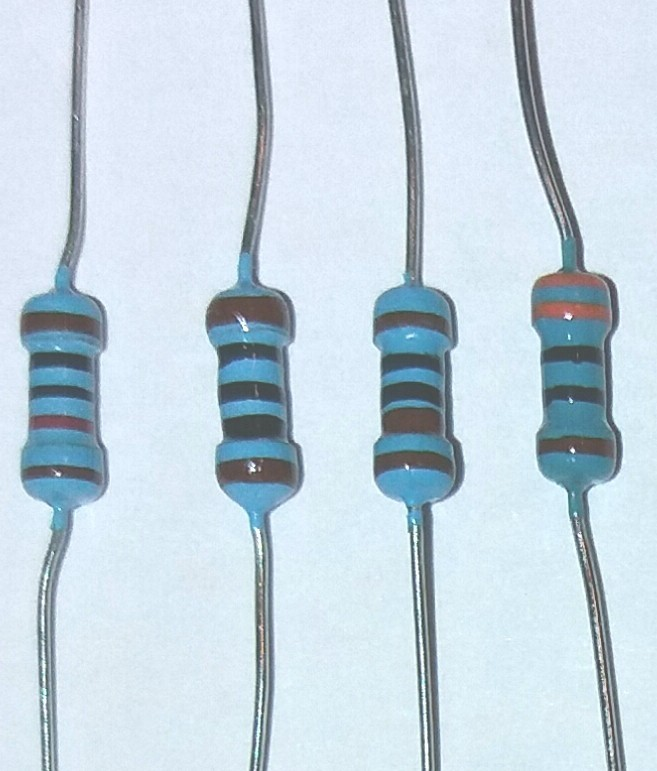
\includegraphics[width=0.9\textwidth,angle=90]{./pics/Widerstaende.jpg}
		\end{minipage}
		\hfill
		\begin{minipage}{0.43\textwidth}
			\centering
			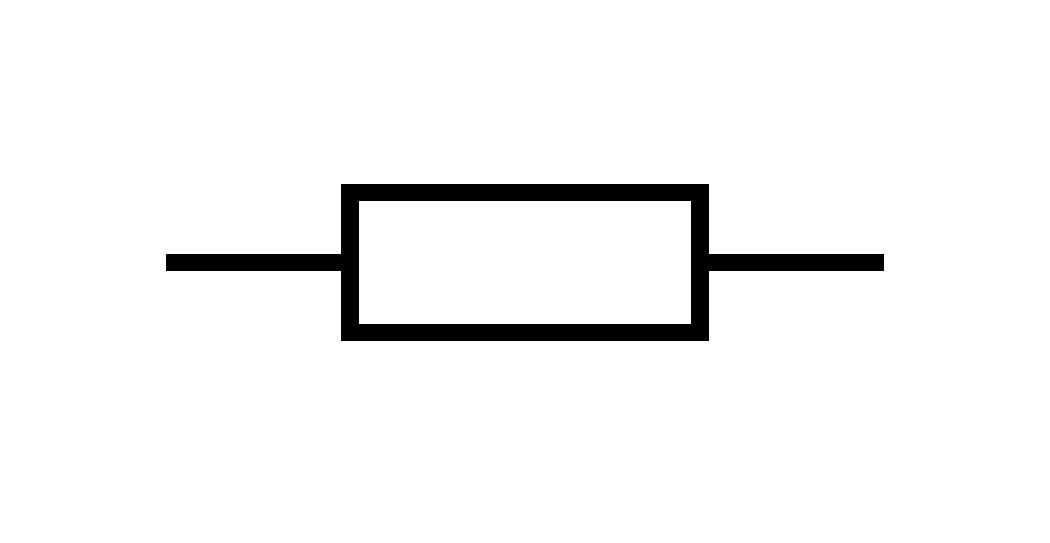
\includegraphics[width=0.8\textwidth]{./Zeichnungen/widerstand-schaltsymbol.png}
		\end{minipage}
	\end{minipage}
\end{zsfg}


\newpage
\section{Vermischte Übungen}

% TODO: Vermischte Übungen ergänzen

\begin{aufgabe} \emph{Farbcodierung von Widerständen}
	
	\begin{enumerate}[label=\alph*), itemsep=0ex]
		\item Gib die Farbcodierung der folgenden Widerstandsgrößen an:
		\begin{multicols}{3}
			\begin{enumerate}[label=(\arabic*)]
				\item $\SI{330}{\ohm} \pm 1\%$,
				\item $\SI{10}{\kilo\ohm} \pm 2\%$,
				\item $\SI{4,7}{\kilo\ohm} \pm 10\%$.
			\end{enumerate}
		\end{multicols}
		\item Gib die Größe der folgenden Widerstände an:
		\begin{multicols}{2}
			\begin{enumerate}[label=(\arabic*)]
				\item 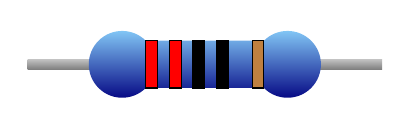
\begin{tikzpicture}[scale=0.3]
				\shade [top color=lightgray, bottom color=gray] (-5,0.8) rectangle (10,1.2);
				\shade [top color=LightSkyBlue, bottom color=NavyBlue] (0,0) -- (5,0) arc [start angle=-135, end angle=135, radius=1.414] -- (0,2) arc [start angle=45, end angle=315, radius=1.414];
				\draw [fill=red] (0,0) rectangle ++(0.5,2);
				\draw [fill=red] (1,0) rectangle ++(0.5,2);
				\draw [fill=black] (2,0) rectangle ++(0.5,2);
				\draw [fill=black] (3,0) rectangle ++(0.5,2);
				\draw [fill=brown] (4.5,0) rectangle ++(0.5,2);
				\end{tikzpicture}
				\item 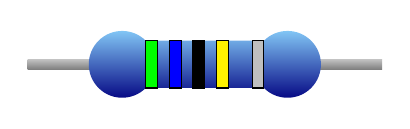
\begin{tikzpicture}[scale=0.3]
				\shade [top color=lightgray, bottom color=gray] (-5,0.8) rectangle (10,1.2);
				\shade [top color=LightSkyBlue, bottom color=NavyBlue] (0,0) -- (5,0) arc [start angle=-135, end angle=135, radius=1.414] -- (0,2) arc [start angle=45, end angle=315, radius=1.414];
				\draw [fill=green] (0,0) rectangle ++(0.5,2);
				\draw [fill=blue] (1,0) rectangle ++(0.5,2);
				\draw [fill=black] (2,0) rectangle ++(0.5,2);
				\draw [fill=yellow] (3,0) rectangle ++(0.5,2);
				\draw [fill=lightgray] (4.5,0) rectangle ++(0.5,2);
				\end{tikzpicture}
			\end{enumerate}
		\end{multicols}
	\end{enumerate}
	\emph{Hinweis:} Als Hilfsmittel ist die Widerstandskarte aus den Boxen zugelassen.
\end{aufgabe}


\vfill


\begin{links}
	\item \href{https://www.youtube.com/watch?v=EbVmfGNwn0g}{FUTUREMAG}
	
	Kurze Dokumentation des FUTUREMAG zur Arduino-Welt
	
	\item \href{https://www.heise.de/make/meldung/Mehr-Komfort-der-Arduino-Ueberkopfwecker-4046184.html}{Arduino-Wecker}
	
	Mit einem selbst gebauten Wecker, der Uhrzeit und Alarmzeit getrennt voneinander anzeigt, erfüllte ein Bastler seinen Wunsch nach mehr Komfort.
	
	\item \href{https://www.instructables.com/id/Aquarium-LED-Controller/}{Aquarium-Licht}
	
	Der Bastler hinter diesem Projekt wollte seinen Fischen im Aquarium ein natürliches Licht einschließlich Sonnenaufgang, Sonnenuntergang und Nacht gönnen. Auf die gleiche Art und Weise kann man natürlich auch sein Terrarium beleuchten.
	
	\item \href{https://www.heise.de/make/meldung/Kein-Geld-fuer-eine-Oculus-Rift-VR-Brille-selbstgebaut-3949507.html}{VR-Brille}
	
	Drei Schüler aus Frankreich hatten kein Geld für eine Virtual Reality Brille – aber dafür das Know How, um sich mit einem Arduino und einem Gehäuse aus dem 3D-Drucker selbst eine VR-Brille zu basteln.
\end{links}


